\documentclass{homework}
\usepackage{homework}
\usepackage{hanhua}
\title{report}
\subtitle{Project A}
\begin{document}
\maketitle
\section{Q1.1}
\subsection{任务}
将一篇英文文章中出现过的所有单词以字典序排列(忽略大小写),并根据每种字符在文章中的出现频率进行Huffman编码(区分大小写)。
\subsection{解决方法}
\subsubsection{按字典序排列}
\begin{enumerate}
    \item 建立26个链表,分别对应26个首字母的字典;
    \item 在扫描文本时对单词进行分割,并将单词一律转为小写;
    \item (关键步骤)将处理后的单词以插入排序法插入对应其首字母的字典中,每次比较用到字典序规则。
    \item 依次打印26个字典(链表)。
\end{enumerate}
\subsubsection{Huffman编码}
\begin{enumerate}
    \item 开辟数组统计所有单字节可打印字符的出现次数,并在扫描文本过程进行统计;
    \item 建立一个储存Huffman树结点的堆,堆顶结点权重最小;
    \item 将出现次数不为0的所有字符作为叶子结点放入堆中,其权重即为出现频率(次数);
    \item (关键步骤)构建Huffman树:每次弹出权重最小的两个节点,将其分别作为左右孩子连接到新建的父亲结点后将父亲重新放入堆中,父亲结点权重为子结点权重之和。反复此步骤直至堆中只有一个根结点;
    \item 编码:遍历已构建的Huffman树并分配编码:根节点编码为空串,左孩子编码为父亲编码加一位'0',右孩子加一位'1';
    \item 按字典序打印所有字符的Huffman编码。
\end{enumerate}
\subsection{函数说明}
\begin{enumerate}
    \item ord // 返回字母序号,A/a为0(为compareWord服务)
    \item compareWord // 返回两单词在字典序中先后顺序(为insertWord服务)
    \item insertWord // 将单词按字典序插入已排序的指定字典中
    \item goLowerCase // 将单词转为全小写
    \item finNindexNcount // 从文件读入,将单词排序,统计字符出现次数
    \item buildHuffman // 构建Huffman树(步骤即“解决方法”中相关部分)
    \item printDict // 打印字典
    \item swapNode // 堆操作:交换堆中两结点位置(为push与pop服务)
    \item push // 堆操作:将结点压入堆中
    \item pop // 堆操作:弹出堆顶结点
    \item combine // Huffman树操作:将两结点作为孩子链接到新建父亲结点
    \item draw // 画树(检查程序用)
    \item assignCode // 遍历Huffman树并分配编码
    \item printHuff // 按字典序打印字符的Huffman编码
\end{enumerate}
\subsection{关键函数复杂度分析}
    \subsubsection{insertWord}
    \paragraph{时间复杂度}若L为单词最大长度,N为文章单词数量,则逐个字符比对的compareWord时间复杂度为$\mathcal{O}(L)$,而insertWord采用从链表头线性逐个比较,符合条件后插入故时间复杂度为$\mathcal{O}(LN)$。最坏情况既所有单词首字母相同且每次插入的单词的字典序都排在最后。可以使用二分查找法插入将时间复杂度降为$\mathcal{O}(L\mathrm{log}N)$,但由于链表旅行操作来回定向反而更费时间,需要使用哈希表储存指针,用空间换取时间,以真正达到上述复杂度。
    \paragraph{空间复杂度}$\mathcal{O}(1)$
    \subsubsection{buildHuffman}
    \paragraph{时间复杂度}buildHuffman函数由两部分组成。第一部分为依次push所有字符,其权重即其出现次数。第二部分为不断合并结点直至成为一颗树,每次合并由两次pop、一次combine和一次push组成。pop为将堆顶元素和最后一个元素对调后将新堆顶元素不断和更小的孩子交换直至堆重新变为最小堆,push则将待插入元素放入堆底并不断和大的父亲交换直至堆变为最小堆,两个函数时间复杂度都为$\mathcal{O}(\mathrm{log}N)$;combine复杂度为$\mathcal{O}(1)$。整个过程需要重复(N-1)次。故buildHuffman时间复杂度为$\mathcal{O}(N\mathrm{log}N+3(N-1)\mathrm{log}N)=\mathcal{O}(N\mathrm{log}N)$
    \paragraph{空间复杂度}$\mathcal{O}(1)$
\subsection{边界情况分析}
\begin{itemize}
    \item 本程序采用逐行读取而非逐字读取,一次性将整行文字读入buff中,便于进行单词分割。然而BUFFSIZE设为了固定的值,若出现越界则超出部分无法读入。事实上若预先检查一下是否越界,若越界则使用realloc扩大buff大小即可,这样在申请的时候不用申请那么大节省了空间,同时也避免了越界问题。
    \item 同样本程序堆的大小HEAPSIZE也固定了,但由于只统计ASCII码为单字节的可打印字符,即ASCII码在30到127之间的字符,故堆大小足够,且也必须。
    \item 每个单词长度的上界WORDLEN设为固定。若考虑输入文本为无意义乱码或单词间隔被删除的情况,应先预处理文本再调用本程序,预处理超出了本程序应该解决的问题范畴。
    \item 字符Huffman编码的长度上限CODELEN也没有问题,最差情况即为Huffman树退化为一个每个结点其中一个儿子都是叶子的情况,也就是字符出现频率形如1,2,4,8这样前面最小的n个加起来也没有第n+1个大的这种情况,考虑所统计字符总数的限制,编码长度不会越界。
    \item 对于其他编码的文字,如UTF-8中汉字等字符需要占用多个字节(一般为3个)储存时,单独解析其中的每一个字节可能会得到无意义的内容,然而第一位符号位为负解决了这个问题(事实上也是由于数组下标出现负数报错而发现了这一情况),所以当碰到字符编码不在所统计范围内时并不报错,只是提出警告并跳过即可。其实这也应属于文本预处理的内容。
\end{itemize}
\subsection{程序运行结果}
下图是将生成的Huffman树打印出来:
\begin{figure}[H]
    \centering
    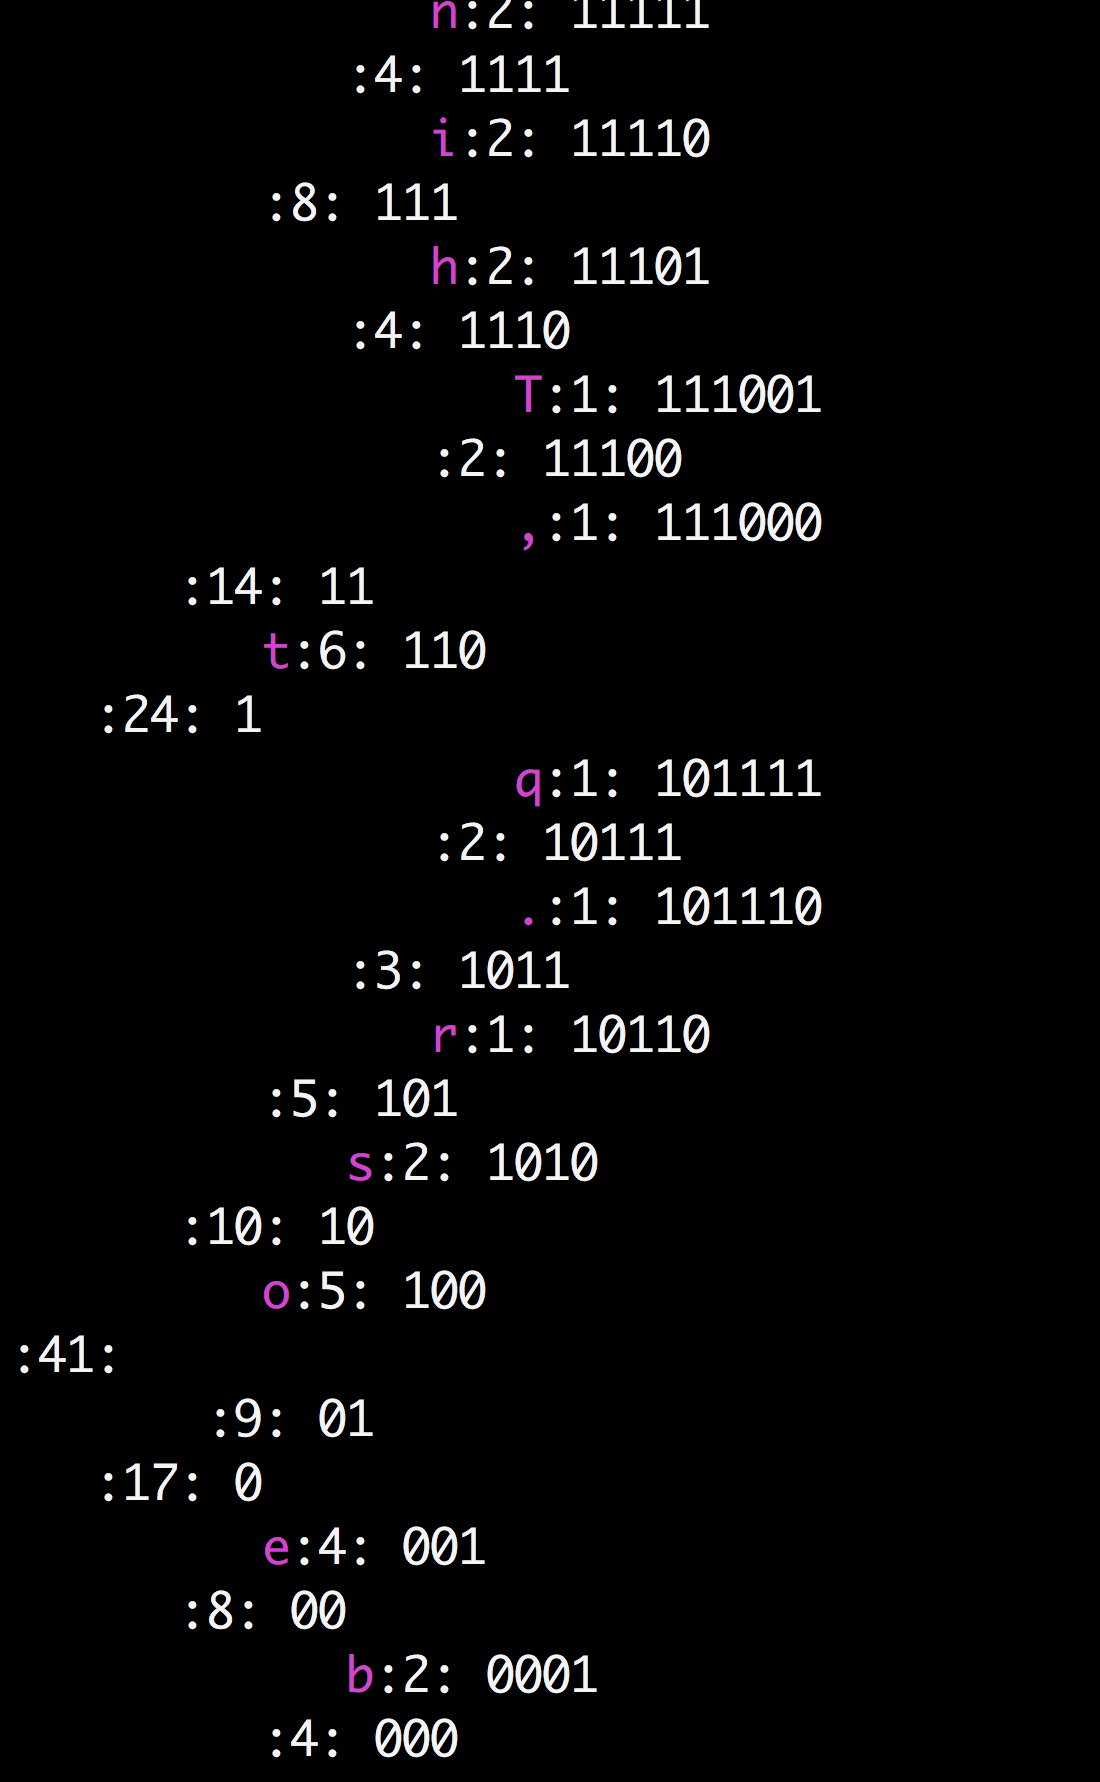
\includegraphics[width=7cm]{Q1.1/tree.png}
\end{figure}
文件夹中input1.txt为Huffman编码的中文维基百科页面中全部内容(包括网页上所有信息),程序处理结果也非常理想,详见Q1.1/dictionary.txt和Q1.1/huffman.txt。
\section{Q1.2}
\subsection{任务}
分别用堆和多链表这两种形式维护一个优先队列,队列中有先来后到的、不同紧急级别的病人,级别高的优先,同级别的先来的优先。病人会来到(enqueue)、中途退出(quit)、更新紧急级别(update),医院需要随时知道下一个该让哪个病人看医生(dequeue),以及所有病人的优先顺序(print)。
\subsection{用堆实现解决方法}
\begin{enumerate}
    \item 堆本身的实现不再赘述。注意quit的病人可能在堆中任意位置,故用一个数组来根据病人ID记录病人在堆中的位置。本质上是一个不太强的哈希表,将病人ID对IDSCALE(本程序为质数1000003)取模后为其储存位置。
    \item quit和dequeue后期对堆重新整理的过程都要用到“将代替其位置的元素不断下滚到合适位置”这一过程,故抽象出来一个函数叫做rollDown。
    \item 为区别同样级别病人,记录病人来到时间,时间随病人来到而增加1,初始为0。
    \item update采用病人先退出,再以更新后级别、更新时时间作为一个新的病人加入排队实现。
    \item print采用先复制整个堆,再依次出队实现。
\end{enumerate}
\subsection{用多链表实现解决方法}
\begin{enumerate}
    \item 动态地为每个级别的病人建立一个双向链表,元素顺序为病人优先顺序。将所有级别的链表头串成一个高级链表,链表头顺序为紧急级别顺序。
    \item 每当新病人出现时,若已有其级别链表则将其插入该链表,若无则在恰当位置建立新链表并插入。
    \item 出队时返回并删除将第一个链表的第一个元素。
    \item 出队或中途离开时,需检查该级别链表是否变为空,若是则需将链表头在高级链表中删除。
    \item 更新级别也采用离开再以新病人加入两部来实现。
    \item 中途离开和更新级别同样用到根据ID储存每个病人指针的办法,快速找到病人位置并进行操作。
\end{enumerate}
\subsection{函数说明}
\begin{enumerate}
    \item goLowerCase // 将单词变全小写(用于对比识别操作指令)
    \item myAtoi // 将字符串转换为整数(处理病人的ID和紧急级别)
    \item isLetterDigit // 返回是否为字母或数字(用于分割输入的各参数)
    \item swapPatient // 交换两病人在堆中位置(为enQ和rollDown服务)
    \item whoRules // 比较两病人优先顺序(见任务描述)
    \item enQ // 将病人加入堆/多链表中
    \item rollDown // 将堆中制定位置病人下滚到合适位置(为deQ和quit服务)
    \item deQ // 返回并删除优先级最高的病人
    \item quitQ // 指定ID病人退出堆/多链表
    \item update // 指定ID病人更新紧急级别
    \item printQ // 按优先顺序打印所有病人
    \item mainLoop // 主循环:读取操作类型、相关参数,并执行操作
\end{enumerate}
\subsection{关键函数复杂度分析}
    \subsubsection{enQ(堆)}
    \paragraph{时间复杂度}N为同时在排队的最大病人数,时间复杂度为$\mathcal{O}(\mathrm{log}N)$。
    \paragraph{空间复杂度}$\mathcal{O}(1)$
    \subsubsection{enQ(多链表)}
    \paragraph{时间复杂度}N为同时在排队的同级别最大病人数,L为紧急级别的数量。需要从高级链表头走到对应级别链表头,再走到队尾,时间复杂度为$\mathcal{O}(L+N)=\mathcal{O}(N)$(因为级别数量不会大于病人数量,即最多每个病人都不同级别)。其实可以记录一下每个级别链表的尾结点指针,这样只用$\mathcal{O}(1)$就可以了,但是需要空间$\mathcal{O}(L)$。
    \paragraph{空间复杂度}$\mathcal{O}(1)$
    \subsubsection{deQ(堆)}
    \paragraph{时间复杂度}N为同时在排队的最大病人数,时间复杂度为$\mathcal{O}(\mathrm{log}N)$。
    \paragraph{空间复杂度}$\mathcal{O}(1)$
    \subsubsection{deQ(多链表)}
    \paragraph{时间复杂度}由于可以直接根据ID找到该病人指针,时间复杂度为$\mathcal{O}(1)$。
    \paragraph{空间复杂度}$\mathcal{O}(1)$
    \subsubsection{quit(堆)}
    \paragraph{时间复杂度}同deQ(堆),时间复杂度为$\mathcal{O}(\mathrm{log}N)$。
    \paragraph{空间复杂度}$\mathcal{O}(1)$
    \subsubsection{quit(多链表)}
    \paragraph{时间复杂度}$\mathcal{O}(1)$。
    \paragraph{空间复杂度}$\mathcal{O}(1)$
    \subsubsection{update(堆)}
    \paragraph{时间复杂度}quit+enQ,时间复杂度为$\mathcal{O}(\mathrm{log}N)$。
    \paragraph{空间复杂度}$\mathcal{O}(1)$
    \subsubsection{update(多链表)}
    \paragraph{时间复杂度}quit+enQ=$\mathcal{O}(N)$。
    \paragraph{空间复杂度}$\mathcal{O}(1)$
    \subsubsection{print(堆)}
    \paragraph{时间复杂度}复制堆需要$\mathcal{O}(N)$,N次deQ需要$\mathcal{O}(N\mathrm{log}N)$,故总时间复杂度为$\mathcal{O}(N\mathrm{log}N)$。
    \paragraph{空间复杂度}$\mathcal{O}(N)$(复制出来的堆)
    \subsubsection{print(多链表)}
    \paragraph{时间复杂度}$\mathcal{O}(N)$
    \paragraph{空间复杂度}$\mathcal{O}(1)$
\subsection{边界情况分析}
\begin{itemize}
    \item 文件读入手段同前一题,故BUFFSIZE分析同前一题,但规范输入不会太长,若假定病人ID和紧急级别都不会超过int整形大小,病人姓名不会超过NAMESIZE(本程序默认为200)。
    \item 在用堆实现中,病人到达时间T也为整形,堆大小HEAPSIZE为1048576。根据经验,即使是北京/上海排队挂号最火热的大医院,一个科室门诊一天最多也就在数千个号这个数量级,所有门诊、急诊加起来也不会超过$10^6$这个数量级,故每天重启程序即可。
    \item 所有dequeue操作皆会判断队列是否为空,所有update、quit均会判断指定ID病人是否存在,其他各种判空情形也在程序中写出,并分别返回警告或错误。
\end{itemize}
\subsection{程序运行结果}
用堆实现:
\begin{figure}[H]
    \centering
    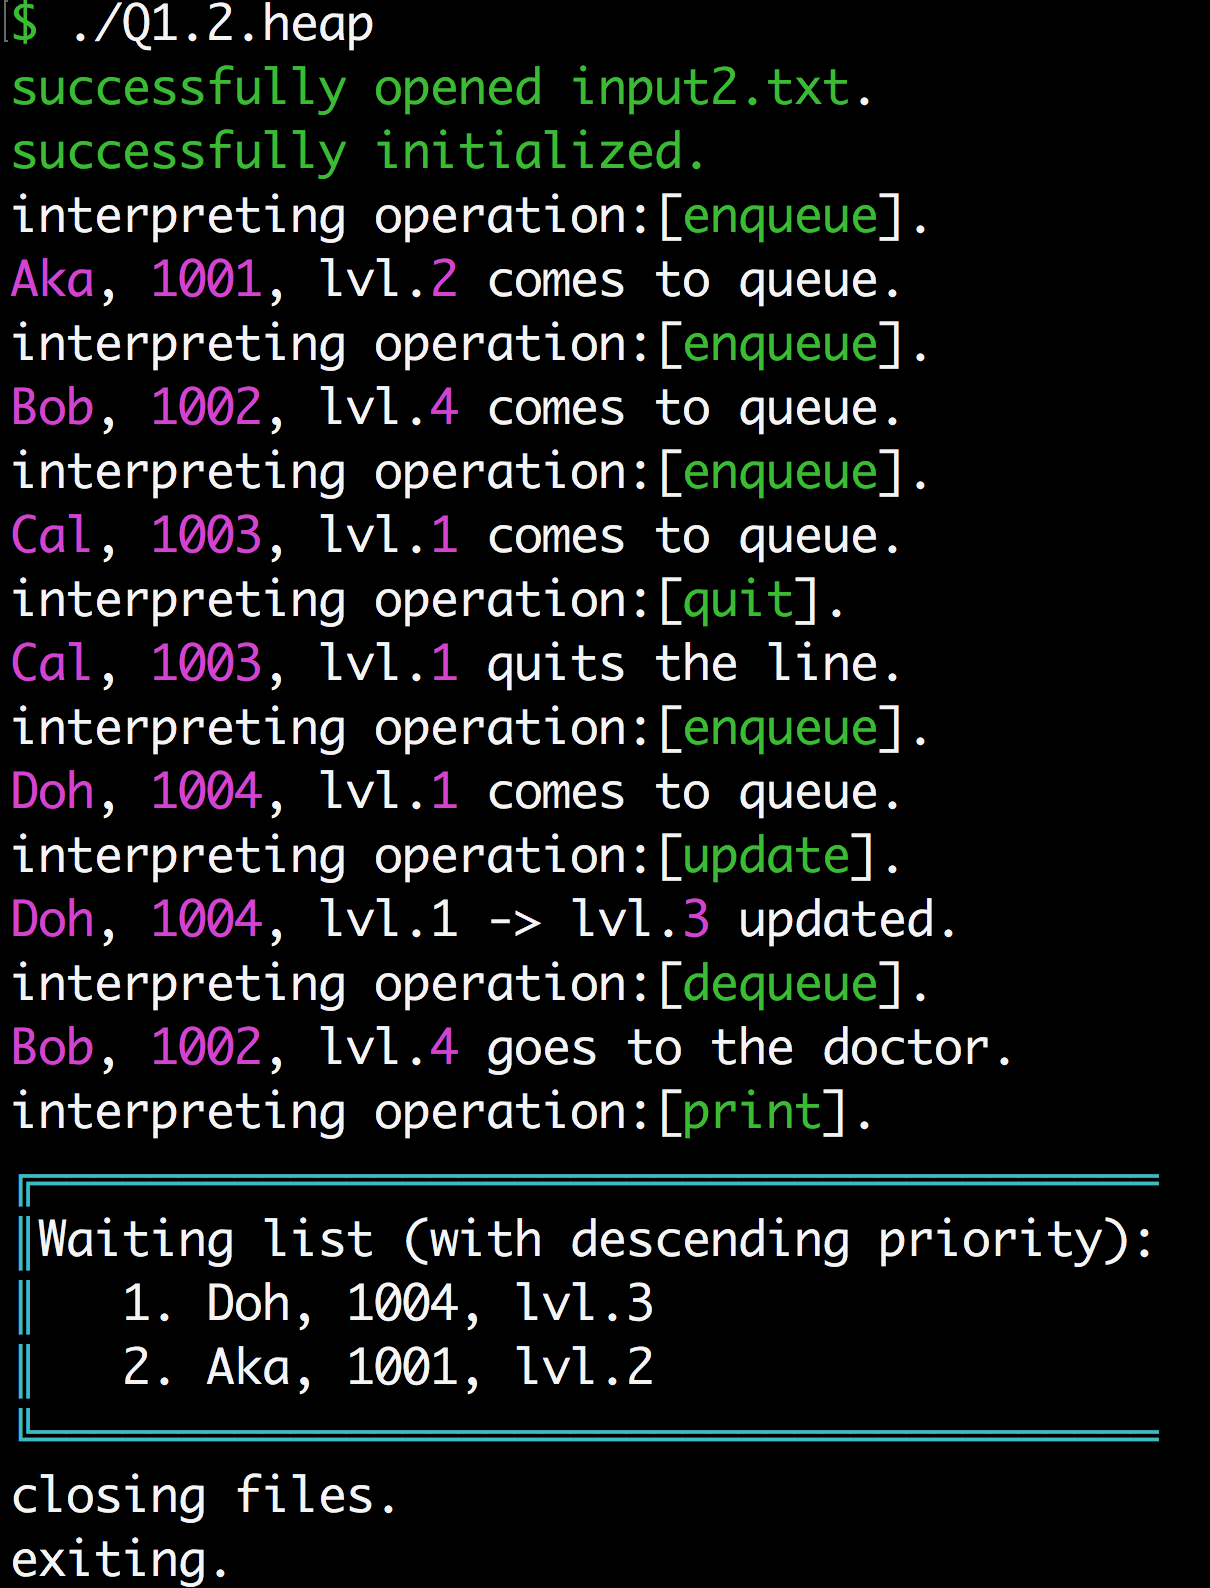
\includegraphics[width=7cm]{Q1.2/Q1.2.heap.png}
\end{figure}
用多链表实现(可以容易判断某级别是否还有病人):
\begin{figure}[H]
    \centering
    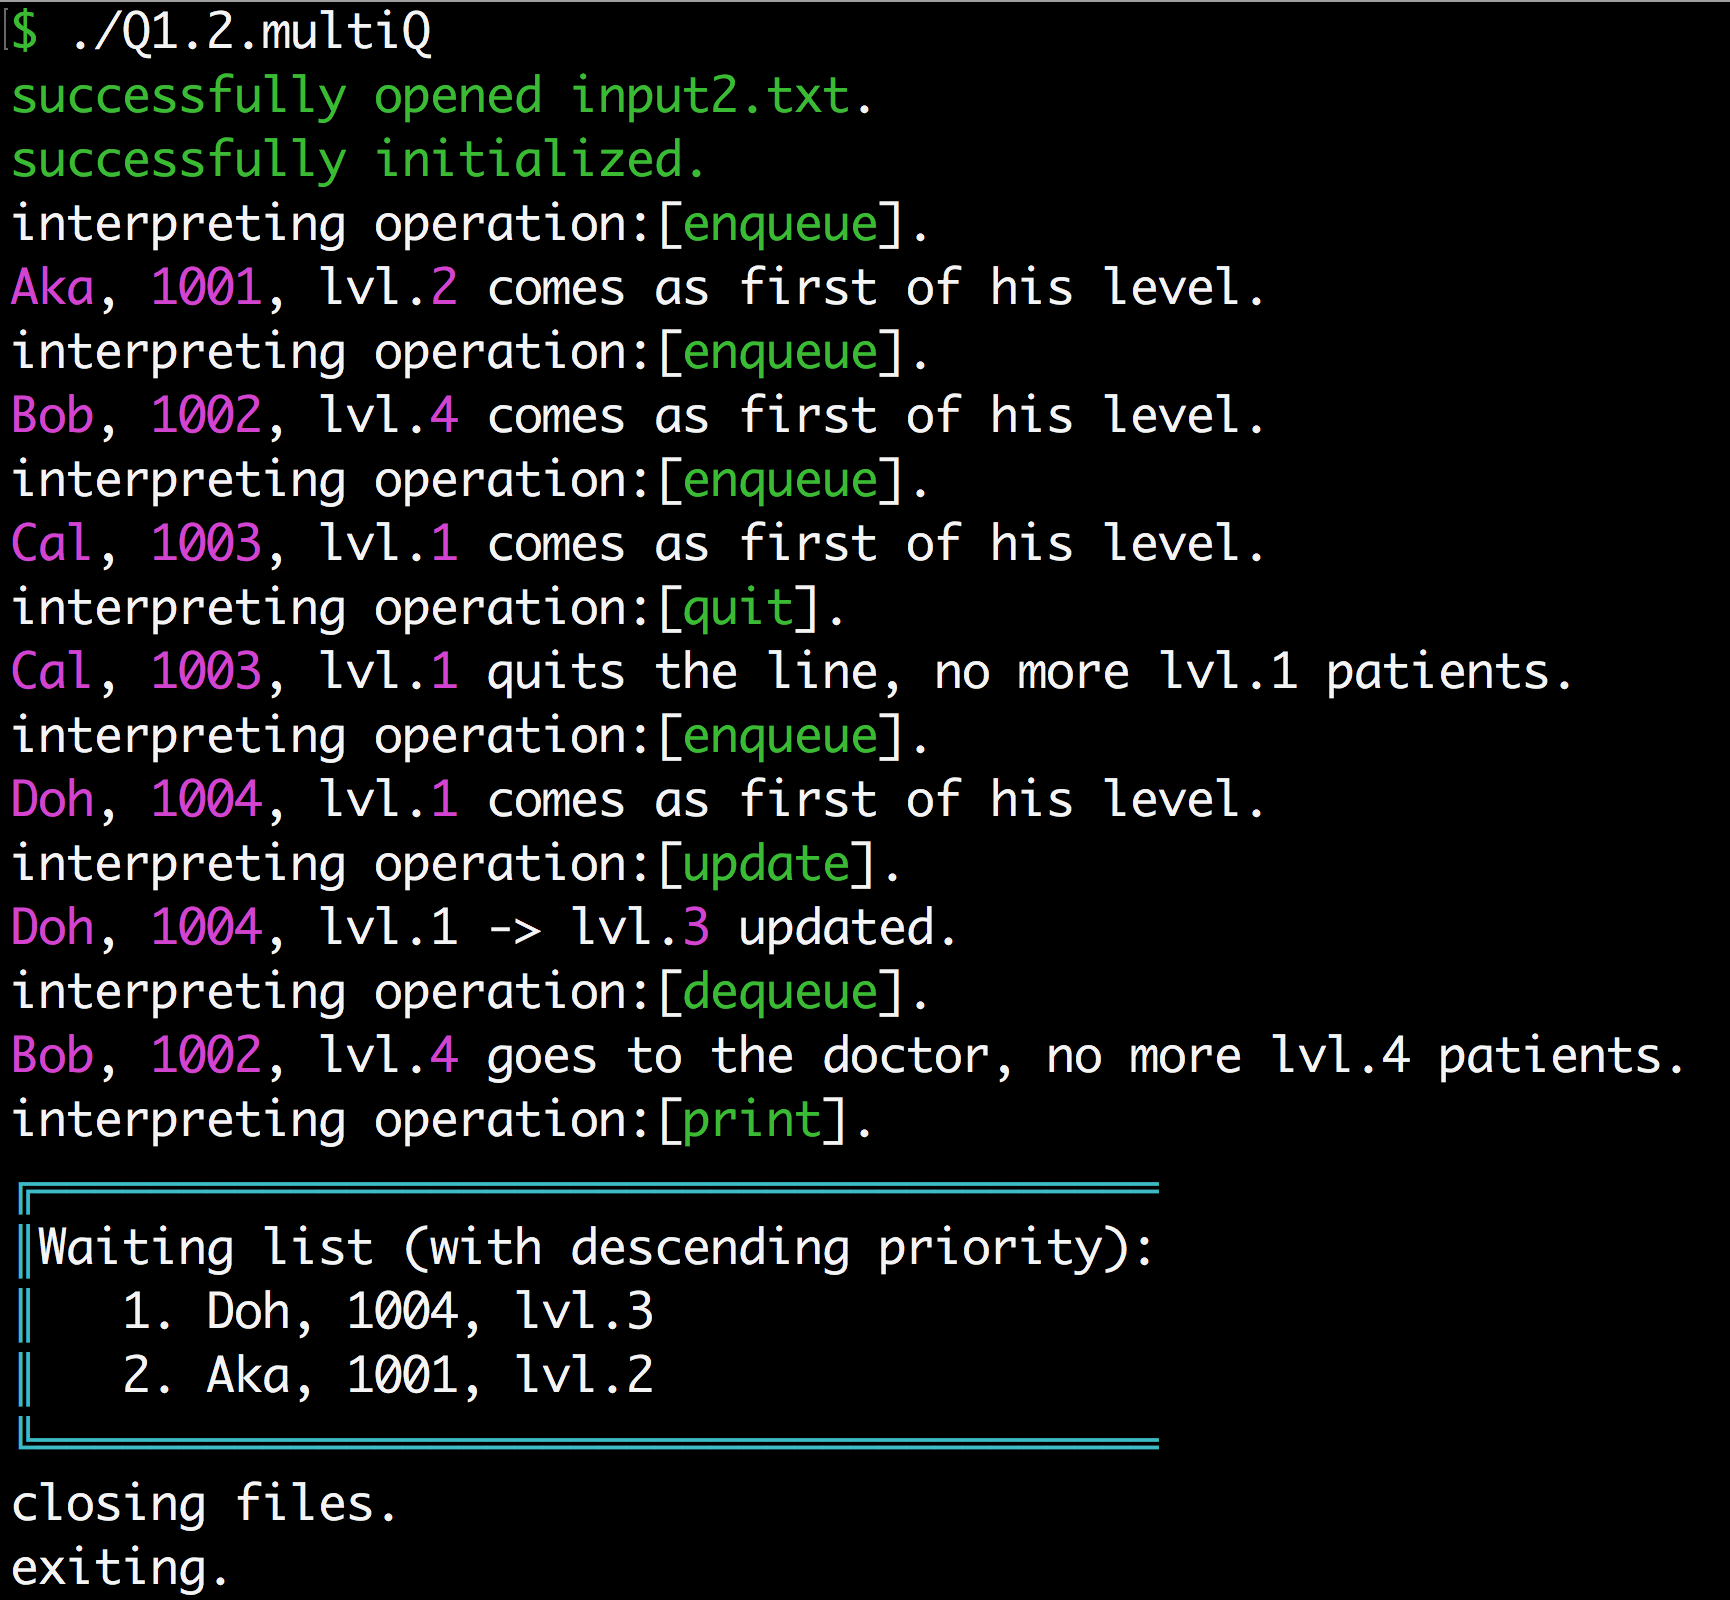
\includegraphics[width=7cm]{Q1.2/Q1.2.multiQ.png}
\end{figure}
\section{Q1.3(报告从略)}
\subsection{任务}
根据二叉树的先序遍历和中序遍历结果重构树,将树镜像翻转,并输出翻转后树的后序遍历结果和双孩子结点个数。
\subsection{解决方法}
重构树:
\begin{enumerate}
    \item 先序遍历结果第一个元素为根节点,在中序遍历中找到他;
    \item 中序遍历中根节点左右串分别为其左右子树,在先序遍历中对应标记他们;
    \item 分别对左右子树的先序遍历和中序遍历结果递归地运用本方法。
\end{enumerate}
翻转树:递归地翻转根节点坐字数和右子树。
\paragraph{说明:}事实上无需翻转树,镜像树的后序遍历结果就是在原本树中:先遍历右子树再遍历左子树再访问根节点的结果。双孩子结点树也不随翻转而变化。
\subsection{程序运行结果}
\begin{figure}[H]
    \centering
    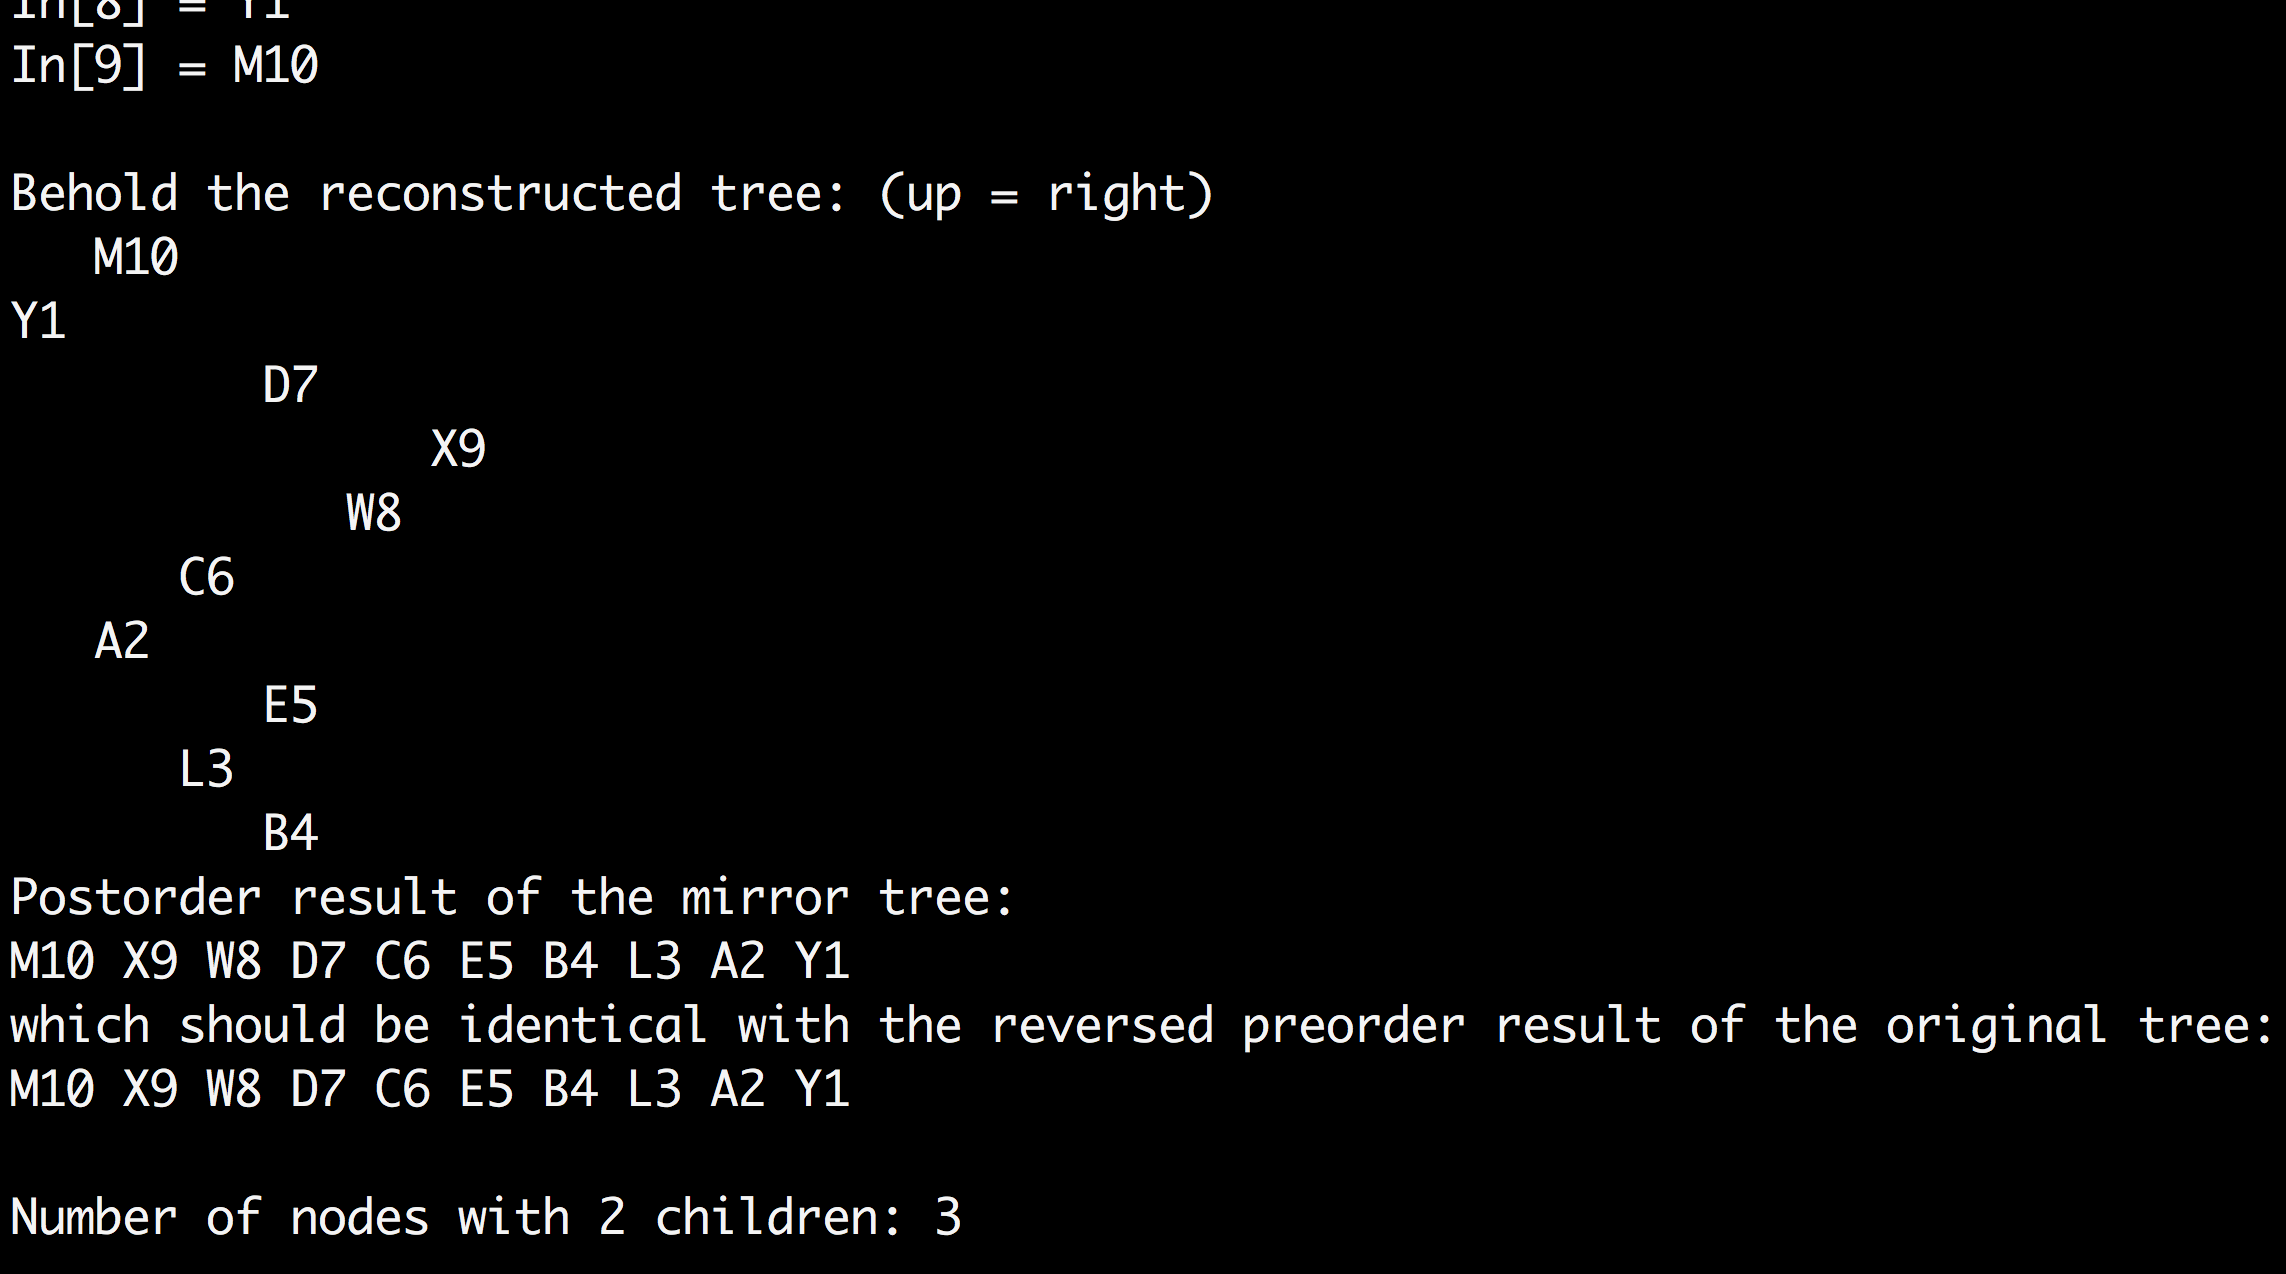
\includegraphics[width=7cm]{Q1.3/mirror.png}
\end{figure}
\section{Q1.4}
\subsection{任务}
读入两个数x、y,输出其和x+y、差x-y、乘积x$\times$y,若第二个数为整数则还要输出幂$x^y$。
\subsection{解决方法}
\subsubsection{加法}
将两数按小数点对齐,从低位到高位逐位相加、进位。(仅处理两个正数)
\subsubsection{减法}
先处理两数大小和符号,通过再次调用加法或减法,然后符号单判断,使得只处理两个正数的大数减小数。

然后同样是按小数点对齐,从低位到高位逐位相减,若出现负数则借位并更新。

因为保证绝对值上是大数减小数,所以无需最后从高位开始检查是否为负数,逐渐向低位回退。
\subsubsection{乘法}
首先计算乘积的小数位数,将两个数转化为整数进行乘法运算,然后再加上小数点和符号。

整数乘法采用karastuba算法:将两个大整数从中间切开,计算高位和低位分别对应相乘结果,计算高位低位之和相乘,再用加减法和移位(十进制)实现原本两数乘法结果的计算。这样只用对原来大整数长度一半长的整数进行乘法运算,递归地调用karastuba算法即可。

在两个数位数均不超过1000时为平凡情况,按照小学竖式乘法运算即可:计算两个数每个位置之间互相乘积并加到结果的对应位上,最后从低位开始向高位进位,再从高位向低位回退前导零位数。
\subsubsection{幂}
若y为偶数,则$x^y=x^{[y/2]}\times x^{[y/2]}$,否则$x^y=x^{[y/2]}\times x^{[y/2]}\times x$,其中$[y]$为不超过y的最大整数(即向下取整)。

按照以上规则递归地调用求幂函数,在0、1、2次方时给出边界情况的答案:1、x、x$\times$x。
\subsection{函数说明}
\begin{enumerate}
    \item initNum // 初始化Num类型:包括数字位数、符号、是否整数、小数点位置及各位数字
    \item readNum // 从字符串指定位置将数读取到指定Num类型
    \item printNum // 打印Num类型(可控制仅屏幕输出或同步输出到文件)
    \item cutNum // 将指定Num类型在指定位置提取片段作为新的Num类型
    \item paste // 左移位:在Num后补零(为multiply服务)
    \item minus // 返回相反数(为substract服务)
    \item compareNum // 比较两数大小(为substract服务)
    \item fracToInt // 将小数转化为整数(为multiply服务)
    \item intToFrac // 将整数在指定位置插入小数点(为multiply服务)
    \item karastuba // 大整数快速乘法的递归实现(multiply主要内容)
    \item divideTwo // 返回除以二向下取整(为power服务)
    \item add // 加法
    \item substract // 减法
    \item multiply // 乘法
    \item power // 幂运算
    \item mainLoop // 主循环:读取x和y,计算并输出所需结果。
\end{enumerate}
\subsection{关键函数复杂度分析}
设N为两个数中位数较长的那个数的位数。
\subsubsection{add, substraction}
\paragraph{时间复杂度} $\mathcal{O}(N)$
\paragraph{空间复杂度} $\mathcal{O}(N)$由于返回的Num类型皆为新开辟的,故此为最少需要空间,下同。
\subsubsection{multiply}
在平凡情况下:
\paragraph{时间复杂度} $\mathcal{O}(N^2)$
\paragraph{空间复杂度} $\mathcal{O}(N)$

调用的karastuba函数,它將兩個n位數字相乘所需的一位數乘法次數減少到了至多$3n^{\log _{2}3}\approx 3n^{1.585}$(引自wiki)而平凡情况用了1000位乘法来加速,故时间复杂度要比$\mathcal{O}(N^2)$小一点。
\subsubsection{power}
\paragraph{时间复杂度} $\mathcal{O}(N^2\mathrm{log}N)$,$N^2$为调用乘法的时间。
\paragraph{空间复杂度} 空间复杂度上,由于每次递归只需要算一次一半幂,实际上可以用尾递归加速,一共要调用$\mathrm{log}N$次,故总空间复杂度为$\mathcal{O}(N\mathrm{log}N)$。
\subsection{边界情况分析}
\begin{itemize}
    \item BUFFSIZE分析,同前;数字位数上界MAXLEN采用固定值(本程序为1048576),因为连续数组无法分配太大空间,但其实同样也可以用链表实现动态大小。
    \item $0^y$强行定义为0,即使是$0^0$。
    \item 在读入数后先将其和0相加,主要是清除前导零、小数点后尾缀零。
\end{itemize}
程序运行结果请见Q1.4/output4.txt。

{\bf 更多精细判断和操作都在程序源代码里啦!辛苦助教老师!}
\end{document}
